\section{Methodology and System Design}
\label{sec:methodology}

The methodological framework designed in this dissertation unites symbolic linguistic engineering with deep representation learning into an end-to-end, multi-stage processing pipeline. The complete system architecture is illustrated in Figure~\ref{fig:architecture}. The framework comprises four interconnected operational tiers: (1) Linguistic Preprocessing and the 83-Rule FST Morphological Engine, (2) Morpho-Contrastive AI Text Detection, (3) Morphologically-Grounded Fact Verification and Hybrid Retrieval, and (4) the Continuous 2D Cartesian Trust Matrix.

\begin{figure*}[t]
\centering
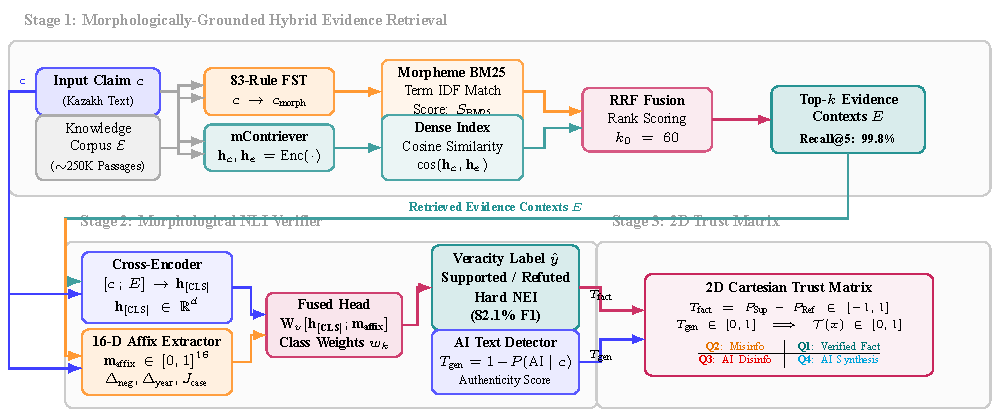
\includegraphics[width=0.98\textwidth]{figures/fig_framework_architecture.pdf}
\caption{End-to-end system architecture for morphologically-grounded fact verification and AI text detection in low-resource agglutinative languages. \textbf{Stage 1}: 83-rule FST stemmer and dense multilingual encoder (\textsc{mContriever}) fused via RRF ($k_0 = 60$) over a 250K passage knowledge corpus. \textbf{Stage 2}: Cross-encoder representation $\mathbf{h}_{[\text{CLS}]}$ fused with the 16-D morphological diagnostic vector $\mathbf{m}_{\text{affix}}$ via class-weighted softmax head ($w_k$). \textbf{Stage 3}: Continuous 2D Trust Matrix mapping factual veracity $T_{\text{fact}}$ and generative authenticity $T_{\text{gen}}$ into four operational risk quadrants.}
\label{fig:architecture}
\end{figure*}

\subsection{Linguistic Preprocessing and the 83-Rule FST Analyzer}
Kazakh grammar adheres to strict phonological and morphotactic constraints, governed by palatal/labial vowel harmony and regressive/progressive consonant assimilation. To model these phenomena deterministically, we implement an 83-rule Finite-State Transducer (FST) rule engine that operates directly over normalized Cyrillic-Kazakh text. 

Given an input string $s$, the transducer applies sequential peeling passes across four canonical inflectional tiers:
\begin{equation}
    s \xrightarrow{\text{FST Pass 1}} s_{\text{case}} \xrightarrow{\text{FST Pass 2}} s_{\text{poss}} \xrightarrow{\text{FST Pass 3}} s_{\text{plur}} \xrightarrow{\text{FST Pass 4}} \mathcal{R}(s)
\end{equation}
where $\mathcal{R}(s)$ denotes the canonical invariant root morpheme. The 83 grammatical rules encode:
\begin{itemize}[leftmargin=*, nosep]
    \item \textbf{Plural Suffixes (6 allomorphs):} \textit{-лар/-лер}, \textit{-дар/-дер}, \textit{-тар/-тер}.
    \item \textbf{Possessive Suffixes (16 allomorphs):} 1st, 2nd (polite/informal), and 3rd person singular and plural markers (\textit{-ым/-ім}, \textit{-ыңыз/-іңіз}, \textit{-сы/-сі}).
    \item \textbf{Case Suffixes (14 allomorphs):} Nominative (unmarked), Accusative (\textit{-ны/-ні/-ды/-ді/-ты/-ті}), Dative (\textit{-ға/-ге/-қа/-ке}), Locative (\textit{-да/-де/-та/-те}), Ablative (\textit{-дан/-ден/-тан/-тен}), Instrumental (\textit{-мен/-бен/-пен}), and Genitive (\textit{-ның/-нің/-дың/-дің/-тың/-тің}).
    \item \textbf{Verbal Negation and Aspect (12 allomorphs):} Root-adjacent unstressed negation infixes (\textit{-ба/-бе/-па/-пе/-ма/-ме}, \textit{-паған/-пеген}).
    \item \textbf{Evidentiality and Modality Markers (8 allomorphs):} Witnessed past (\textit{-ды/-ді}), indirect evidential past (\textit{-ыпты/-іпті}, \textit{екен}), and necessity/possibility modal operators (\textit{керек}, \textit{тиіс}, \textit{мүмкін}).
\end{itemize}

From the extracted morphological parses, the system constructs a continuous 16-dimensional morphological diagnostic vector $\mathbf{m}_{\text{affix}} \in [0, 1]^{16}$ for any claim-evidence pair $(c, E)$:
\begin{equation}
    \mathbf{m}_{\text{affix}} = \left[ m_1, m_2, \dots, m_{16} \right]^\top
\end{equation}
The vector specifically encodes: (1) Lexical and surface length ratios ($m_1$); (2) Directional negation mismatch $m_2 = \Delta_{\text{neg}} = |N_c - N_e|$; (3) Disjoint 4-digit calendar year conflicts $m_3 = \Delta_{\text{year}} = \mathbb{I}(\mathcal{Y}_c \cap \mathcal{Y}_e = \emptyset)$; (4) Quantitative numerical disparity $m_4 = \Delta_{\text{num}}$; (5--8) Evidentiality and epistemic modality mismatches (witnessed vs.\ reportative vs.\ speculative); (9) FST root Jaccard overlap $m_9 = J_{\text{root}} = \frac{|\mathcal{R}_c \cap \mathcal{R}_e|}{|\mathcal{R}_c \cup \mathcal{R}_e|}$; (10) Raw surface token overlap $m_{10} = J_{\text{surf}} = \frac{|\mathcal{S}_c \cap \mathcal{S}_e|}{|\mathcal{S}_c \cup \mathcal{S}_e|}$; (11) Inflectional divergence $\Delta_{\text{div}} = |J_{\text{surf}} - J_{\text{root}}|$; (12) Syntactic case root overlap $m_{12} = J_{\text{case}}$; and (13--16) Proper-noun coreference and sequence bounds.

\subsection{Morpho-Contrastive AI Text Detection Module}
To distinguish machine-generated Kazakh text from human-authored prose, we construct a Morpho-Contrastive detection network trained on a newly curated Tri-Domain dataset spanning 9,000 documents:
\begin{itemize}[leftmargin=*, nosep]
    \item \textbf{News Domain:} 3,000 articles from verified Kazakh journalistic agencies (Tengrinews, Kazinform, Azattyq).
    \item \textbf{Academic/Encyclopedic Domain:} 3,000 articles from the Kazakh Wikipedia repository.
    \item \textbf{Social/Conversational Domain:} 3,000 posts from Twitter, Telegram, and consumer discussion boards.
\end{itemize}
Machine-generated counterparts are synthesized using state-of-the-art LLMs, including GPT-4o, LLaMA-3-8B-Instruct, Mistral-7B, and Sherkala-7B (the leading open Kazakh foundation model).

The network encodes input text through a multilingual transformer backbone (\textsc{XLM-RoBERTa-large}) to produce contextual sequence embedding $\mathbf{h}_{[\text{CLS}]} \in \mathbb{R}^{d}$. Simultaneously, the 83-rule FST computes the morpheme frequency distribution vector $\mathbf{v}_{\text{morph}} \in \mathbb{R}^{K}$. Both representations are projected into a shared metric embedding space $\mathbf{z} = \text{MLP}([\mathbf{h}_{[\text{CLS}]}; \mathbf{W}_m \mathbf{v}_{\text{morph}}])$. Training optimizes a joint objective combining Supervised Contrastive Loss ($\mathcal{L}_{\text{SupCon}}$) \cite{khurana2023contrastive} and Cross-Entropy ($\mathcal{L}_{\text{CE}}$):
\begin{equation}
    \mathcal{L}_{\text{total}} = \mathcal{L}_{\text{CE}} + \lambda \, \mathcal{L}_{\text{SupCon}}
\end{equation}
\begin{equation}
    \mathcal{L}_{\text{SupCon}} = \sum_{i \in I} \frac{-1}{|P(i)|} \sum_{p \in P(i)} \log \frac{\exp(\mathbf{z}_i \cdot \mathbf{z}_p / \tau)}{\sum_{a \in A(i)} \exp(\mathbf{z}_i \cdot \mathbf{z}_a / \tau)}
\end{equation}
where $P(i)$ denotes positive instances sharing the same origin label (human vs.\ machine), and $\tau = 0.07$ is a temperature hyperparameter. The network outputs the generative authenticity score $T_{\text{gen}} \in [0, 1]$:
\begin{equation}
    T_{\text{gen}} = 1 - P(\text{AI-Generated} \mid c)
\end{equation}

\subsection{Morphologically-Grounded Fact Verification Pipeline}
The factual verification tier operates across a curated knowledge corpus of 250,000 passage chunks extracted from Kazakh Wikipedia and public fact-checking archives (Factcheck.kz).

\paragraph{Hybrid Evidence Retrieval (Stage 1)}
To guarantee high evidence recall despite inflectional variance, retrieval fuses sparse lexical search and dense semantic representations:
\begin{enumerate}[leftmargin=*, label=(\alph*)]
    \item \textit{Morpheme-Stemmed BM25}: Input queries are parsed through the 83-rule FST stemmer, mapping inflected tokens to canonical root lemmas: $c \to c_{\text{morph}}$. Standard BM25 scoring is computed over an inverted index of pre-stemmed passages:
    \begin{equation}
        S_{\text{BM25}}(c, e) = \sum_{t \in c_{\text{morph}}} \text{IDF}(t) \cdot \frac{f(t, e_{\text{morph}}) \cdot (k_1 + 1)}{f(t, e_{\text{morph}}) + k_1 \left(1 - b + b \cdot \frac{|e_{\text{morph}}|}{\text{avgdl}}\right)}
    \end{equation}
    \item \textit{Dense Neural Retrieval (\textsc{mContriever})}: Unsupervised multilingual dense representations compute bi-encoder cosine similarity:
    \begin{equation}
        S_{\text{dense}}(c, e) = \cos(\mathbf{h}_c, \mathbf{h}_e) = \frac{\text{Enc}(c) \cdot \text{Enc}(e)}{\|\text{Enc}(c)\| \|\text{Enc}(e)\|}
    \end{equation}
    \item \textit{Reciprocal Rank Fusion (RRF)}: Candidate rankings are merged via RRF ($k_0 = 60$) \cite{cormack2009rrf}:
    \begin{equation}
        \text{RRF}(e) = \frac{1}{k_0 + \text{Rank}_{\text{BM25}}(e)} + \frac{1}{k_0 + \text{Rank}_{\text{dense}}(e)}
    \end{equation}
\end{enumerate}

\paragraph{Cross-Encoder Verification (Stage 2)}
The top-$k$ retrieved evidence sentences ($E = \{e_1, \dots, e_k\}$) and the claim $c$ are concatenated as a cross-encoder input sequence: $[c \,;\, E] \to \mathbf{h}_{[\text{CLS}]} \in \mathbb{R}^d$. The contextual representation $\mathbf{h}_{[\text{CLS}]}$ is concatenated with the 16-D morphological diagnostic vector $\mathbf{m}_{\text{affix}}$ and projected through a linear classification head:
\begin{equation}
    P(y \mid c, E) = \text{softmax}\left(\mathbf{W}_v \left[\mathbf{h}_{[\text{CLS}]}; \mathbf{m}_{\text{affix}}\right] + \mathbf{b}_v\right)
\end{equation}
To counteract class imbalance, training optimizes weighted cross-entropy:
\begin{equation}
    \mathcal{L}_{\text{NLI}} = - \sum_{k=1}^3 w_k \cdot y_k \log P(y = k \mid c, E)
\end{equation}
with inverse-frequency weights $w_{\textsc{Sup}} = 0.735$, $w_{\textsc{Ref}} = 1.307$, $w_{\textsc{NEI}} = 0.958$.

\subsection{Continuous 2D Cartesian Trust Matrix Formulation}
To deliver actionable auditing intelligence, we formulate the continuous 2D Trust Matrix $\mathcal{T} = [-1, 1] \times [0, 1]$. We define the \textbf{Factual Veracity Score} $T_{\text{fact}} \in [-1, 1]$ as the calibrated difference between entailment and contradiction probabilities:
\begin{equation}
    T_{\text{fact}} = P(\textsc{Supported} \mid c, E) - P(\textsc{Refuted} \mid c, E)
\end{equation}
where $T_{\text{fact}} > 0$ denotes verified support, $T_{\text{fact}} < 0$ signifies refutation, and $T_{\text{fact}} \approx 0$ reflects insufficient evidence (\textsc{NEI}).

The \textbf{Generative Authenticity Score} $T_{\text{gen}} \in [0, 1]$ represents the probability of human authorship (Eq.~5). The unified scalar \textbf{Trust Metric} $\mathcal{T}(x) \in [0, 1]$ integrates both dimensions:
\begin{equation}
    \mathcal{T}(x) = \sqrt{\frac{1}{2} \left( \max(0, T_{\text{fact}})^2 + T_{\text{gen}}^2 \right)}
\end{equation}
The continuous space induces four operational risk quadrants:
\begin{itemize}[leftmargin=*, nosep]
    \item \textbf{Quadrant 1 (Q1: Verified Human Ground Truth):} $T_{\text{fact}} > 0, T_{\text{gen}} \ge 0.5$ (Low Risk / Authoritative).
    \item \textbf{Quadrant 2 (Q2: Human Misinformation):} $T_{\text{fact}} \le 0, T_{\text{gen}} \ge 0.5$ (Factual Error / Bias).
    \item \textbf{Quadrant 3 (Q3: AI Disinformation):} $T_{\text{fact}} \le 0, T_{\text{gen}} < 0.5$ (Critical Threat / Synthetic Deception).
    \item \textbf{Quadrant 4 (Q4: AI Synthetic Knowledge):} $T_{\text{fact}} > 0, T_{\text{gen}} < 0.5$ (Synthesized Truth / Needs Attributed Audit).
\end{itemize}
